\section{}


\begin{frame}
\titlepage
\end{frame}

\begin{frame}{Problématique}
\begin{alert}{D'après le ministère de la Santé : }
Il y a eu plus de \textbf{31 millions} d'appels d'urgence en 2018. Seuls \textbf{69\%} des appels étaient décrochés dans la minute.
\end{alert}
\begin{block}{Objectif}
Utiliser la reconnaissance vocale par réseau de neurones pour aider à classifier rapidement l'objet d'un appel.
\end{block}
\end{frame}



\begin{frame}{Les étapes de la reconnaissance automatique de la parole}
\begin{tabular}{ l || c | c | }
    1 & Le traitement acoustique  & 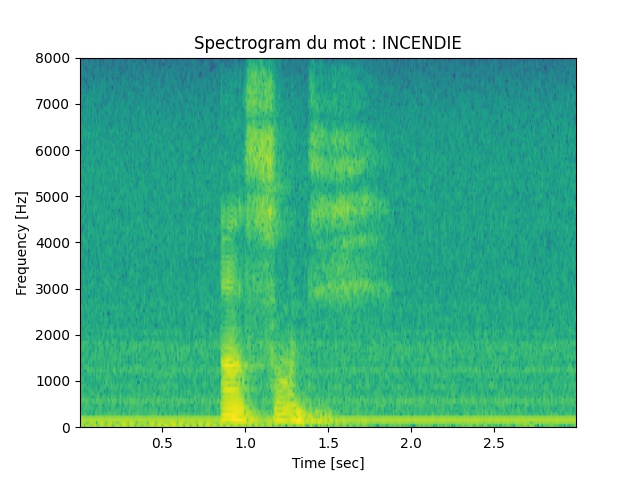
\includegraphics[height=50px]{1-Incendie-3.jpg} \\ \hline \\
    2 & L'apprentissage automatique & 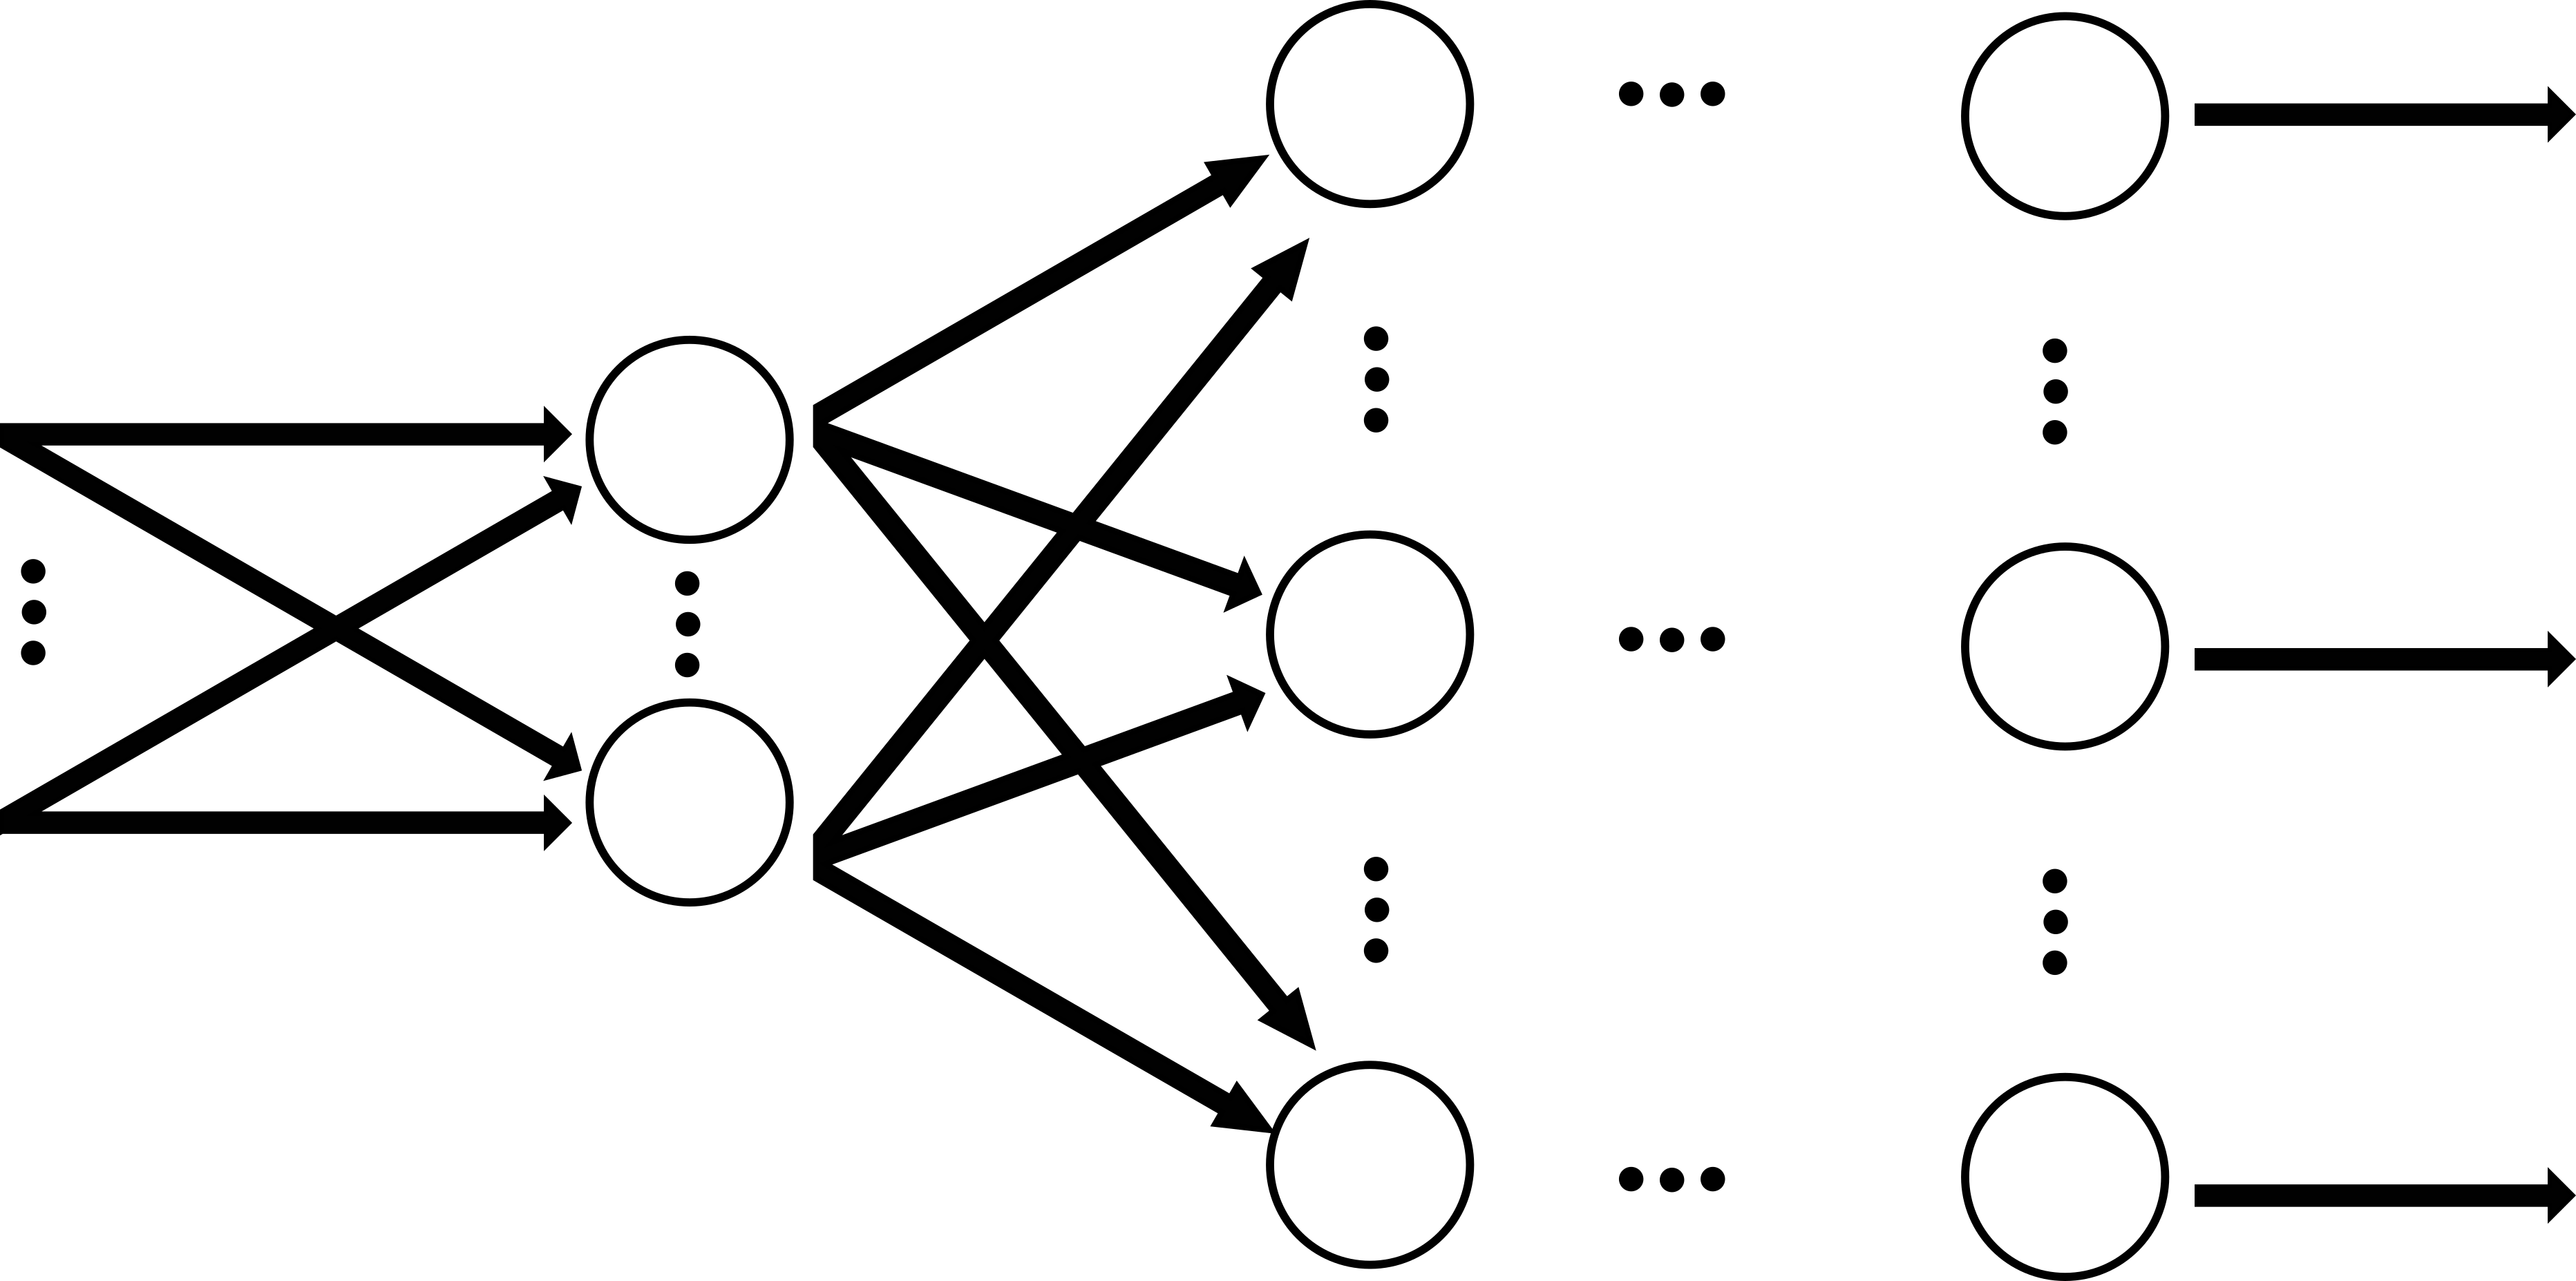
\includegraphics[height=50px]{2-Reseau.png} \\ \hline \\
    3 & Le décodage & 
\includegraphics[height=50px]{3-Matching.png} \\ \hline \\

\end{tabular}
\end{frame}




\begin{frame}{II - Représentation informatique}
\begin{figure}
	\centering
    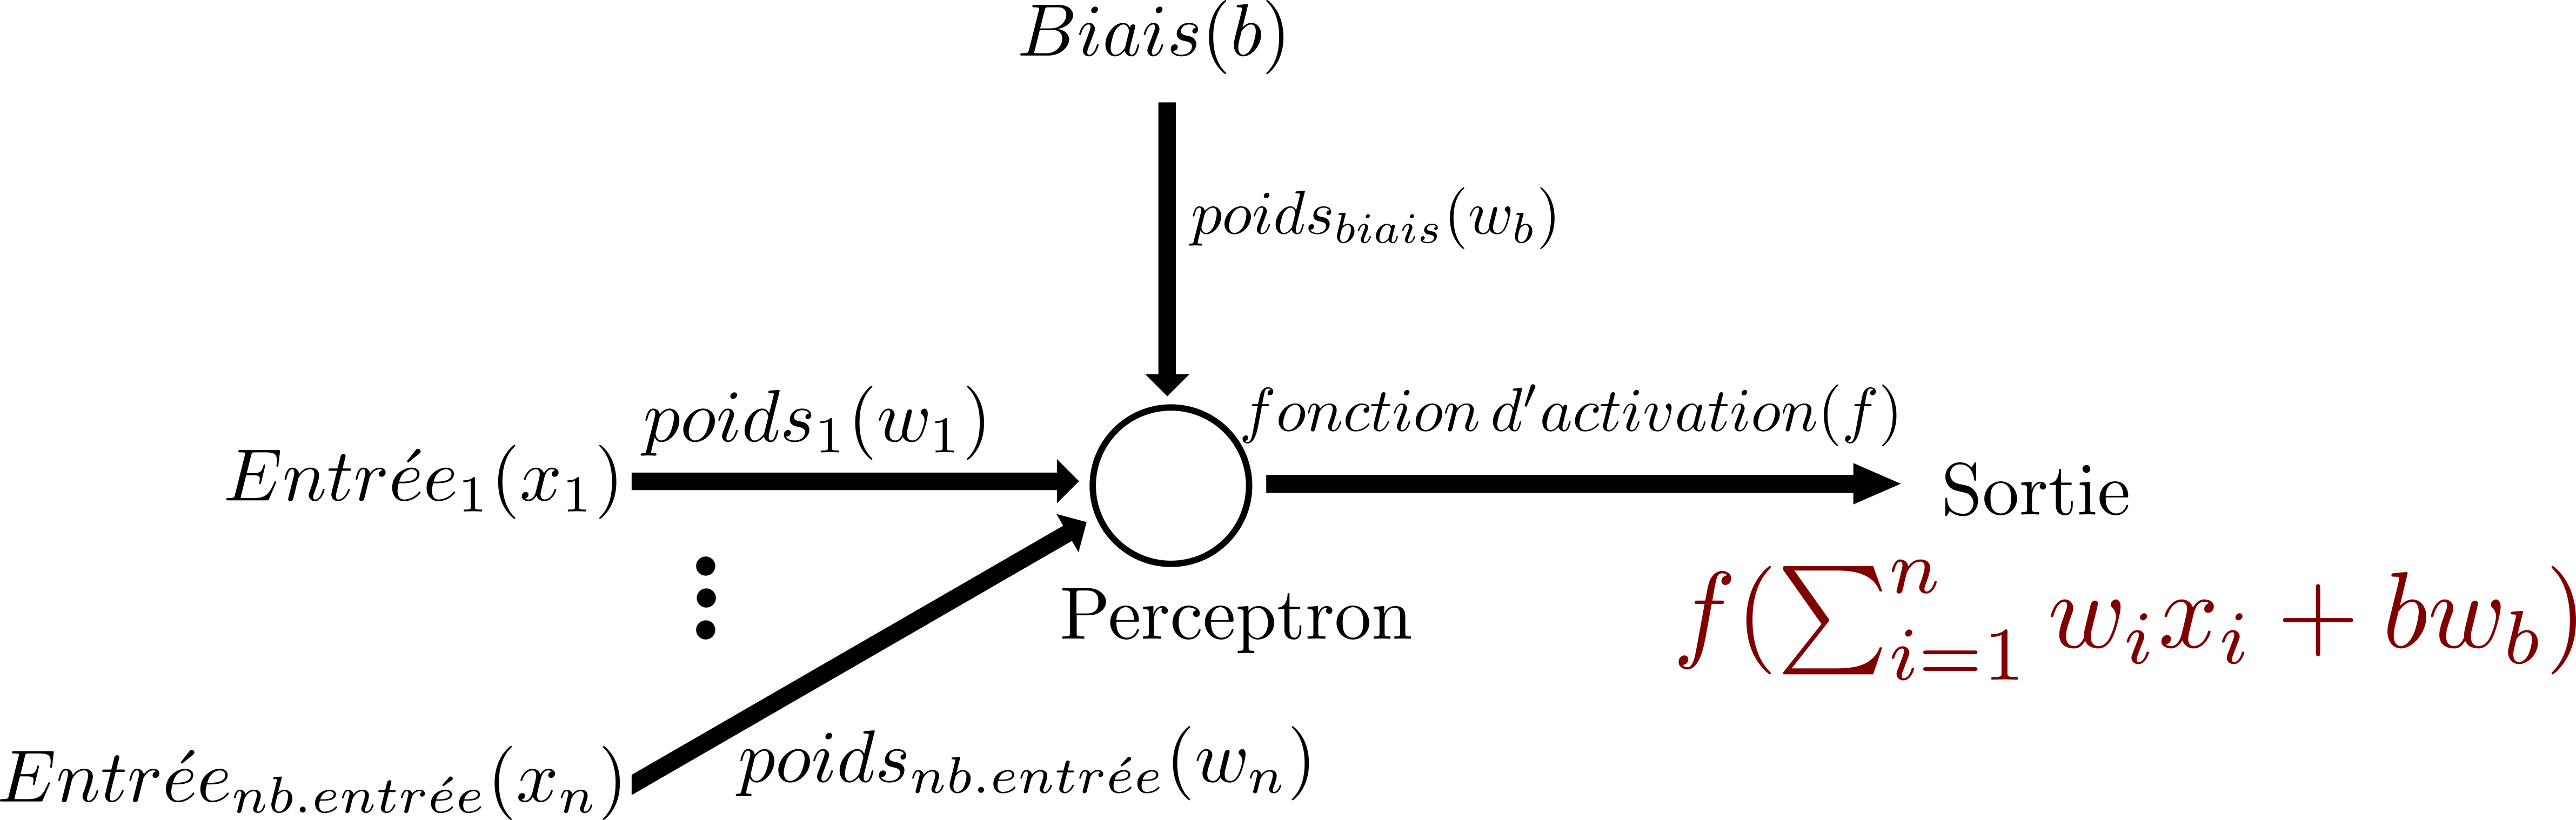
\includegraphics[height=75px]{1-Perceptron.png}
	\caption{Schéma d'un perceptron}	
\end{figure}
\begin{multicols}{2}
$
f
\left(
\begin{pmatrix}
x_1 & \ldots & x_n & b
\end{pmatrix}
\times
\begin{pmatrix}
w_1 \\
\vdots \\
w_n \\
w_b
\end{pmatrix}
\right)
$ \\
La complexité est en $O(n)$
\columnbreak
\lstinputlisting[language=Python]{code.py}
\end{multicols}
\end{frame}